
\begin{comment}

Architecture
@property decorator, lazy evaluation
presented on different layers
    - Drawing
    - Edge
    - Shared properties
    
Feature types - drawing-related, edge-related, shared - kinematic, anomaly describing features

Feature Scope 


Number of nodes in the tree = (N^L-1) / (N-1) 
N - branching factor
L - tree depth

1 + 30 + 30 * 3 + 30 * 3 * 3 + 30 * 3 * 3 * 3

= 1 + a + a*b + a*b^2 + a*b^3

% Higher-level features can be obtained from already available features and added to the feature vector; for example, for the study of diseases the feature 'Age' is useful and is defined as Age = 'Year of death' minus 'Year of birth' . This process is referred to as feature construction.[2][3] Feature construction is the application of a set of constructive operators to a set of existing features resulting in construction of new features. Examples of such constructive operators include checking for the equality conditions {=, ≠}, the arithmetic operators {+,−,×, /}, the array operators {max(S), min(S), average(S)} as well as other more sophisticated operators, for example count(S,C)[4] that counts the number of features in the feature vector S satisfying some condition C or, for example, distances to other recognition classes generalized by some accepting device. Feature construction has long been considered a powerful tool for increasing both accuracy and understanding of structure, particularly in high-dimensional problems.[5] Applications include studies of disease and emotion recognition from speech.[6]


% Main purpose of feature generation phase is to acquire 

% In machine learning and pattern recognition, a feature is an individual measurable property or characteristic of a phenomenon being observed.[1] Choosing informative, discriminating and independent features is a crucial step for effective algorithms in pattern recognition, classification and regression. Features are usually numeric, but structural features such as strings and graphs are used in syntactic pattern recognition. The concept of "feature" is related to that of explanatory variable used in statistical techniques such as linear regression.

% In pattern recognition and machine learning, a feature vector is an n-dimensional vector of numerical features that represent some object. Many algorithms in machine learning require a numerical representation of objects, since such representations facilitate processing and statistical analysis. When representing images, the feature values might correspond to the pixels of an image, while when representing texts the features might be the frequencies of occurrence of textual terms. Feature vectors are equivalent to the vectors of explanatory variables used in statistical procedures such as linear regression. Feature vectors are often combined with weights using a dot product in order to construct a linear predictor function that is used to determine a score for making a prediction.

% utilized and yielded number of local extrema inside corresponding vector of numeric values.


% In the current context, \textit{Drawing} is whole Luria pattern, which consists of line-segments, each represented by vector of points $[p_i, p_{i+1}, ... p_{j-1}, p_j]$ where $[p_i, p_j]$ are starting and ending points of the segment. So the whole \textit{Drawing} is represented by vector of points $[p_1, p_{2}, ... p_{n-1}, p_n]$, where $n$ is total number of points in the Drawing. Subsequent Table \ref{features-drawing} demonstrates subset of \textit{Drawing-related} features, final names are defined by adding prefix constant 'drawing' to following feature names.

\end{comment}

\section{Feature Generation}

Main purpose of current implementation phase is to define and generate features, or individual measurable characteristics of the \textit{Drawing} object or researched Luria pattern for subsequent statistical analysis and creation of classifier model. 

Since discrimination power of particular feature is unknown, it is crucial to construct as many features as possible to produce accurate classifier. Features should also be informative, since it was planned to build individual prediction interpreter model using \textit{"Local Interpretable Model-Agnostic Explanations" (LIME)} algorithm. 

Following sections will describe aspects of technical implementation, methodology, feature indexing and naming, along with feature groups and individual features.

\subsection{Methodology}

It was decided from the scratch not to use straightforward naive approach for feature generation. Features are not generated and evaluated during separate iterative process, but described as computations over internal state of the entity (in our case --- \textit{Drawing} and \textit{Edge} entities) in declarative manner using Python \textit{@property} decorator and evaluated \textit{lazily} in runtime on demand. \textit{Lazy} evaluation is the computational strategy which postpones the evaluation of an expression until its value is actually required (non-strict evaluation).

Also \textit{memoization} technique was applied. \textit{Memoization} is an optimization strategy to speed up computations by storing the results of expensive function calls and returning the cached result, when same inputs occur again. In our case --- if feature evaluation happened, actual value of the feature is cached with possibility to re-trigger evaluation any time. All these aspects provide great computational flexibility and data integrity while working with massive amount of objects. Also it may give the ability to define potentially \textit{infinite} tree-like graphs. Features can be added, changed or even deleted any time on entity level, which immediately affects all nodes of the whole graph. 


\subsection{Edge Naming and Indexing}

Usually we are splitting each \textit{Edge} into three \textit{Edge} sub-objects \textit{[1, 2, 3]}, which describe \textit{[starting, middle, ending]} parts of the certain element of the pattern and also stored as local index of the edge. Given information of graph \textit{depth}, local \textit{index}, \textit{parent} node from the \textit{Edge} object, we can easily construct meaningful index and also deconstruct any index to human-understandable \textit{Edge} description.

\begin{table}[htb]
    \begin{tabular}{p{0.35\linewidth} | p{0.55\linewidth} }
        \hline
        \textbf{Edge Name} & \textbf{Interpretation} \\
        \hline
        edge\_2 & Second stroke of the pattern \\ 
        edge\_2\_1 & Start of the second stroke of the pattern \\ 
        edge\_2\_1\_3 & Ending of the start of the second stroke of the pattern \\ 
        edge-2\_1\_3\_2 & Middle of the ending of the start of second stroke of the pattern \\ 
        \hline
    \end{tabular}
    \caption{Edge Entity --- Naming and Indexing}
\end{table}

\subsection{Feature Engineering}

% Higher-level features can be obtained from already available features and added to the feature vector; for example, for the study of diseases the feature 'Age' is useful and is defined as Age = 'Year of death' minus 'Year of birth' . This process is referred to as feature construction.[2][3] Feature construction is the application of a set of constructive operators to a set of existing features resulting in construction of new features. Examples of such constructive operators include checking for the equality conditions {=, ≠}, the arithmetic operators {+,−,×, /}, the array operators {max(S), min(S), average(S)} as well as other more sophisticated operators, for example count(S,C)[4] that counts the number of features in the feature vector S satisfying some condition C or, for example, distances to other recognition classes generalized by some accepting device. Feature construction has long been considered a powerful tool for increasing both accuracy and understanding of structure, particularly in high-dimensional problems.[5] Applications include studies of disease and emotion recognition from speech.[6]

Feature engineering is a process of application of function set to a set of existing features resulting in creation of new higher-order feature. It is possible to discriminate functions into three categories: 

\begin{easylist}

& Unary functions --- functions, which take one argument, produce single feature from single feature. Sample unary functions would be --- \textit{trigonometric, square root, exponentiation}. 

& Binary functions --- functions, which take two arguments, produce single feature from two features. Sample binary functions would be all arithmetic functions --- \textit{sum, minus, multiplication}.

& Array functions --- multiple-argument functions, produce single feature from array of features. For example --- statistical functions \textit{max, min, median} 

\end{easylist}


In our case, \textit{Drawing} object consists of \textit{Edges}, \textit{Edge} is an array of data points, data point itself is an array of \textit{[x, y, t, p, l, a]} scalar values. 
So any array-like feature of the \textit{Edge} or \textit{Drawing} object can be transformed into higher-order numeric feature by applying statistical functions such as \textit{[mean, median, min, max, standard deviation, $1_{st}$ percentile, $99_{th}$ percentile, ...]}. From \textit{[x, y]} coordinates of data points and time \textit{[t]} we can produce arrays of geometric and kinematic features, such as: \textit{length, height, width, angle, duration, speed, acceleration, jerk} and similarly apply statistical functions to them and once more obtain unique higher-order features. 

\subsection{Feature Naming}

% \begin{table}[htb]
%     \begin{tabular}{p{0.35\linewidth} | p{0.55\linewidth}}
%         \hline
%         Feature & Description \\
%         \hline
        
%         edge\_3\_2\_1\_longitude\_mean & 
%         Average longitude pencil angle of the start of the middle of the third \textit{Edge} of the pattern\\
%         edge-2-1-pressure-max & 
%         Maximum pressure of the start of the second \textit{Edge} of the pattern\\
%         edge-2-3-1-angle & 
%         Angle of the start of the end of the second \textit{Edge} of the pattern\\
%         edge-2-length & 
%         Length of the second \textit{Edge} of the pattern\\
%         drawing-pressure-median & 
%         Median pressure of the \textit{Drawing}\\
%         \hline
        
%     \end{tabular}
%     \caption{Feature Global Names --- Sample Subset}
%     \label{features-higher-order}
% \end{table}


\textit{Feature} is always evaluated in the scope of certain \textit{entity} \textit{[Drawing, Edge]}, by applying certain \textit{function}, therefore global \textit{identification name} of feature is generated by concatenating three main components \textit{[Entity name, Feature name, Function name]}:
\begin{easylist}

& Entity name --- \textit{Edge} entity is named according to relative position in the graph. However \textit{Drawing} is essentially a singleton in the current context.
& Feature name --- concrete feature name.
& Function name --- optional name, used in case of higher-order feature.

\end{easylist}

% Examples of named features along with descriptions are presented in above Table \ref{features-higher-order}. 

% So any \textit{Edge} object can also be described with statistical functions of: \textit{[mean, median, min, max, standard deviation, $1_{st}$ percentile, $99_{th}$ percentile, ...]}. From edge coordinates \textit{[x, y]} and time \textit{[t]} we can produce different geometric and kinematic features, such as: length, height, width, angle, duration, speed, acceleration, jerk.

% It is feasible to combine statistical functions [mean, median, ...] $N_s$, number of describing functions [length, angle, duration, pressure ...] $N_d$, initial number of edges $e_0$ in drawing, number of sub-edges on each level $e$, graph depth $d$ and get possible number of features: $N = e_0 \times (e ^ d) \times N_s \times N_d$

\section{Feature Classes}

\subsection{Edge Features}

    \begin{comment}
    
        angle
        distance
        duration
        speed
        pressure_median
        pressure_max
        pressure_min
        longitude_median
        longitude_max
        longitude_min
        latitude_median
        latitude_max
        latitude_min
    
    \end{comment}

Edge features are defined in the scope of corresponding \textit{Edge} entity. In the context of Luria pattern, \textit{Edge} is line-segment, represented by vector of points $[p_i, p_{i+1}, ... p_{j-1}, p_j]$ where $[p_i, p_j]$ are starting and ending points of the segment. Next Table \ref{features-edge} demonstrates subset of \textit{Edge-related} features, final names are defined by adding variable prefixes to following feature names. Prefix is produced from corresponding name of the \textit{Edge} instance.

\begin{table}[htb]
\centering
\begin{tabular}{p{0.35\linewidth} | p{0.55\linewidth}}
\hline
Edge Feature & Description \\
\hline
angle & Angle of the line between points $[p_i, p_j]$ \\
distance & Euclidean distance between points $[p_i, p_j]$ \\
duration & Time interval between points $[p_i, p_j]$ \\
speed & Linear speed between points $[p_i, p_j]$ \\
pressure\_median & Median pressure in vector of points $[p_i, p_{i+1}..., p_{j-1}, p_j]$ \\
pressure\_max & Max pressure in vector of points \\
pressure\_min & Min pressure in vector of points \\
longitude\_median & Median longitude of a pencil in vector of points \\
longitude\_max & Max longitude of a pencil in vector of points \\
longitude\_min & Min longitude of a pencil in vector of points \\
latitude\_median & Median latitude of a pencil in vector of points \\
latitude\_max & Max latitude of a pencil in vector of points \\
latitude\_min & Min latitude of a pencil in vector of points \\
\hline
\end{tabular}
\caption{Edge Features --- Sample Subset}
\label{features-edge}
\end{table}

\subsection{Drawing Features}

    \begin{comment}
    
        drawing_width
        drawing_length
        drawing_area
        drawing_number_of_strokes
        drawing_number_of_edges
        drawing_completeness
        angle_upper_regression_line
        angle_lower_regression_line
        angle_middle_regression_line
        angle_between_upper_lower_regression_line
    
    \end{comment}

\textit{Drawing-related} features are defined and evaluated in the scope of corresponding \textit{Drawing} entity. In the current context, \textit{Drawing} is whole Luria pattern, which consists of line-segments, each represented by vector of points $[p_i, p_{i+1}, ... p_{j-1}, p_j]$ where $[p_i, p_j]$ are starting and ending points of the segment. So the whole \textit{Drawing} is represented by vector of points $[p_1, p_{2}, ... p_{n-1}, p_n]$, where $n$ is total number of points in the Drawing. Subsequent Table \ref{features-drawing} demonstrates subset of \textit{Drawing-related} features, final names are defined by adding prefix constant 'drawing' to following feature names.

\begin{table}[htb]
\centering
\begin{tabular}{p{0.35\linewidth} | p{0.55\linewidth}}
\hline
Drawing Feature & Description  \\
\hline
width  & Horizontal distance of the \textit{Drawing} $x_{max} - x_{min}$  \\
height & Vertical distance of the \textit{Drawing} $y_{max} - y_{min}$ \\
area & \textit{Drawing} \textit{height} multiplied by \textit{width}  \\
number\_of\_strokes & Number of strokes. Corresponds to maximum stroke \textit{index} in vector of points $[p_1, p_{2}, ... p_{n-1}, p_n]$ \\
number\_of\_edges & Number of \textit{Edge} elements in the Drawing, calculated from number of \textit{Edges} in graph on depth level $d = 0$ \\
completeness & Ratio between \textit{actual} and \textit{expected} number of \textit{Edge} elements in the \textit{Drawing} pattern. Expected number of \textit{Edges} is Luria pattern-type related \textit{constant} \\
angle\_upper\_regression\_line & Angle of \textit{upper} regression line  \\
angle\_lower\_regression\_line & Angle of \textit{lower} regression line  \\
angle\_middle\_regression\_line & Angle of \textit{middle} regression line  \\
angle\_upper\_lower & Angle between \textit{upper} and \textit{lower} regression lines of the \textit{Drawing}\\
\hline
\end{tabular}
\caption{Drawing Features --- Sample Subset}
\label{features-drawing}
\end{table}

To define asymmetry measure of particular Luria pattern, it was decided to construct regression lines from \textit{[upper, middle, lower]} corner nodes of the Drawing and evaluate angle values of corresponding lines. Classification task of extraction \textit{[upper, middle, lower]} nodes, was solved by creating linear regression model from all existing corner nodes, which represents \textit{middle regression line}. During next step, each corner node y-coordinate was compared to y-coordinate of middle regression line, so all corner nodes above \textit{middle regression line} were classified as upper-type. Or lower-type in the opposite case. Similarly, u\textit{pper and lower linear regression lines} were constructed and angle features evaluated. Result is illustrated on Figure \ref{regression-lines}.

\begin{figure}[htb]
  \centering
    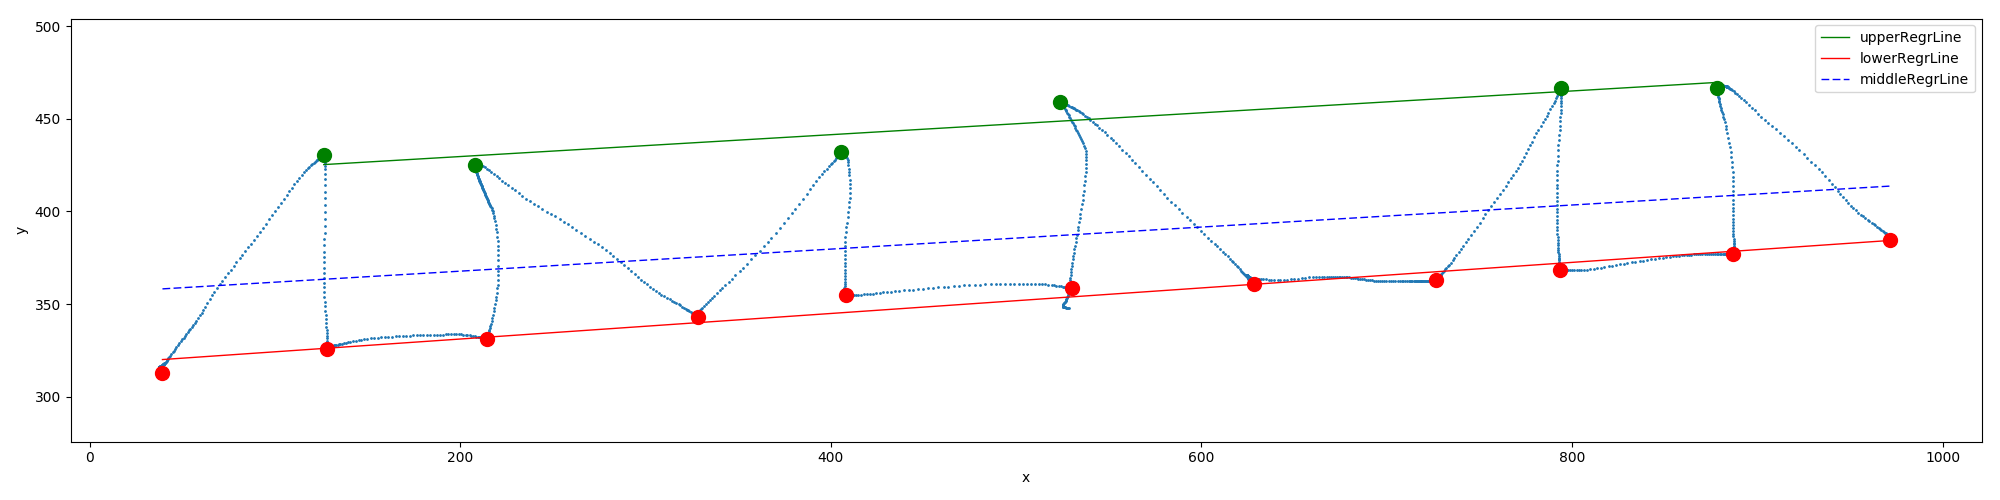
\includegraphics[width=0.99\textwidth]
        {images/features/angle-features}
    \caption{Drawing Features --- \textit{Upper, middle, lower regression lines}}
    \label{regression-lines}
\end{figure}


\subsection{Kinematic and Pressure Features}

\textit{Kinematic} and \textit{pressure} characteristics of handwriting are described in various recent research papers of \citet{zham2017distinguishing, san2016digitized, nomm2016quantitative} and have proven high level of discrimination power between Parkinson's disease patients and healthy subjects. {Kinematic} and \textit{pressure} feature set describes arbitrary vector of points $[p_1, p_{2}, ... p_{n-1}, p_n]$, therefore can be defined and evaluated in the scope of both \textit{Drawing} and \textit{Edge} entities. \textit{Velocity, acceleration, jerk} and \textit{pressure} higher-order features are described and used in subsequent analysis and classifier creation.

Along with standard \textit{[median, mean, mass]} features, another higher-order feature was proposed --- \textit{number of changes}. To evaluate \textit{number of changes}, standard function \textit{argrelextrema()} of \textit{Scipy} library was applied, which is sliding-window based function and yields local \textit{extrema} of the arbitrary array. In our case --- number of \textit{extrema} points within feature vector corresponds to \textit{number of changes} of particular \textit{kinematic} or \textit{pressure} feature.

Following Table \ref{features-kinematic} denotes subset of \textit{kinematic} and \textit{pressure} features. Final names are generated by adding variable prefixes to feature names. Prefix is produced from corresponding name of the \textit{Edge} or \textit{Drawing} instance.


\begin{table}[htb]
\centering
\begin{tabular}{p{0.35\linewidth} | p{0.55\linewidth}}
\hline
Feature & Description \\
\hline
duration & Time period between first and last point of vector $[p_1, p_{2}, ... p_{n-1}, p_n]$\\
trajectory\_length & Sum of all Euclidean distances between all neighbour points in vector \\
velocity\_mass & Velocity mass of the point vector $[p_1, p_{2}, ... p_{n-1}, p_n]$ \\
velocity\_mean & Average velocity of the point vector \\
velocity\_nc & Number of velocity changes in point vector \\
acceleration\_mass & Acceleration mass of the point vector \\
acceleration\_mean & Average acceleration of the point vector \\
acceleration\_nc & Number of acceleration changes in point vector \\
jerk\_mass & Jerk mass of the point vector \\
jerk\_mean & Average jerk of the point vector \\
jerk\_nc & Number of changes in jerk of point vector \\
pressure\_diff\_mean & Average difference in pressure between neighbour points \\
pressure\_mass & Pressure mass of the point vector \\
pressure\_nc & Number of changes in pressure \\
\hline
\end{tabular}
\caption{Kinematic and Pressure Features --- Sample Subset}
\label{features-kinematic}
\end{table}

% \subsection{Sequences of Features}

%     \begin{comment}
    
%     Time series data
%     Streaming data
%     Sequential data
    
%     - Investigate sequences
    
%     (add picture)
    
%     \end{comment}

% Research subject of current thesis is drawing patterns, patterns consist of repetitive elements, in our case - \textit{Edge} object, each \textit{Edge} object possesses certain features. therefore it is good idea to get a clue, how these features progress in time.

